%----------------------------------------------------------------------------------------
%	PACKAGES AND OTHER DOCUMENT CONFIGURATIONS
%----------------------------------------------------------------------------------------

\documentclass[11pt]{article}

%%%%%%%%%%%%%%%%%%%%%%%%%%%%%%%%%%%%%%%%%
% Lachaise Assignment
% Structure Specification File
% Version 1.0 (26/6/2018)
%
% This template originates from:
% http://www.LaTeXTemplates.com
%
% Authors:
% Marion Lachaise & François Févotte
% Vel (vel@LaTeXTemplates.com)
%
% License:
% CC BY-NC-SA 3.0 (http://creativecommons.org/licenses/by-nc-sa/3.0/)
% 
%%%%%%%%%%%%%%%%%%%%%%%%%%%%%%%%%%%%%%%%%

%----------------------------------------------------------------------------------------
%	PACKAGES AND OTHER DOCUMENT CONFIGURATIONS
%----------------------------------------------------------------------------------------

\usepackage{amsmath,amsfonts,stmaryrd,amssymb} % Math packages

\usepackage{enumerate} % Custom item numbers for enumerations

\usepackage[ruled]{algorithm2e} % Algorithms

\usepackage[framemethod=tikz]{mdframed} % Allows defining custom boxed/framed environments

\usepackage{listings} % File listings, with syntax highlighting
\lstset{
	basicstyle=\ttfamily, % Typeset listings in monospace font
}
\usepackage{booktabs}
\usepackage[sort&compress,numbers]{natbib}
%----------------------------------------------------------------------------------------
%	DOCUMENT MARGINS
%----------------------------------------------------------------------------------------

\usepackage{geometry} % Required for adjusting page dimensions and margins

\geometry{
	paper=a4paper, % Paper size, change to letterpaper for US letter size
	top=2.5cm, % Top margin
	bottom=3cm, % Bottom margin
	left=2.5cm, % Left margin
	right=2.5cm, % Right margin
	headheight=14pt, % Header height
	footskip=1.5cm, % Space from the bottom margin to the baseline of the footer
	headsep=1.2cm, % Space from the top margin to the baseline of the header
	%showframe, % Uncomment to show how the type block is set on the page
}

%----------------------------------------------------------------------------------------
%	FONTS
%----------------------------------------------------------------------------------------

\usepackage[utf8]{inputenc} % Required for inputting international characters
\usepackage[T1]{fontenc} % Output font encoding for international characters

\usepackage{XCharter} % Use the XCharter fonts

%----------------------------------------------------------------------------------------
%	COMMAND LINE ENVIRONMENT
%----------------------------------------------------------------------------------------

% Usage:
% \begin{commandline}
%	\begin{verbatim}
%		$ ls
%		
%		Applications	Desktop	...
%	\end{verbatim}
% \end{commandline}

\mdfdefinestyle{commandline}{
	leftmargin=10pt,
	rightmargin=10pt,
	innerleftmargin=15pt,
	middlelinecolor=black!50!white,
	middlelinewidth=2pt,
	frametitlerule=false,
	backgroundcolor=black!5!white,
	frametitle={Command Line},
	frametitlefont={\normalfont\sffamily\color{white}\hspace{-1em}},
	frametitlebackgroundcolor=black!50!white,
	nobreak,
}

% Define a custom environment for command-line snapshots
\newenvironment{commandline}{
	\medskip
	\begin{mdframed}[style=commandline]
}{
	\end{mdframed}
	\medskip
}

%----------------------------------------------------------------------------------------
%	FILE CONTENTS ENVIRONMENT
%----------------------------------------------------------------------------------------

% Usage:
% \begin{file}[optional filename, defaults to "File"]
%	File contents, for example, with a listings environment
% \end{file}

\mdfdefinestyle{file}{
	innertopmargin=1.6\baselineskip,
	innerbottommargin=0.8\baselineskip,
	topline=false, bottomline=false,
	leftline=false, rightline=false,
	leftmargin=2cm,
	rightmargin=2cm,
	singleextra={%
		\draw[fill=black!10!white](P)++(0,-1.2em)rectangle(P-|O);
		\node[anchor=north west]
		at(P-|O){\ttfamily\mdfilename};
		%
		\def\l{3em}
		\draw(O-|P)++(-\l,0)--++(\l,\l)--(P)--(P-|O)--(O)--cycle;
		\draw(O-|P)++(-\l,0)--++(0,\l)--++(\l,0);
	},
	nobreak,
}

% Define a custom environment for file contents
\newenvironment{file}[1][File]{ % Set the default filename to "File"
	\medskip
	\newcommand{\mdfilename}{#1}
	\begin{mdframed}[style=file]
}{
	\end{mdframed}
	\medskip
}

%----------------------------------------------------------------------------------------
%	NUMBERED QUESTIONS ENVIRONMENT
%----------------------------------------------------------------------------------------

% Usage:
% \begin{question}[optional title]
%	Question contents
% \end{question}

\mdfdefinestyle{question}{
	innertopmargin=1.2\baselineskip,
	innerbottommargin=0.8\baselineskip,
	roundcorner=5pt,
	nobreak,
	singleextra={%
		\draw(P-|O)node[xshift=1em,anchor=west,fill=white,draw,rounded corners=5pt]{%
		Question \theQuestion\questionTitle};
	},
}

\newcounter{Question} % Stores the current question number that gets iterated with each new question

% Define a custom environment for numbered questions
\newenvironment{question}[1][\unskip]{
	\bigskip
	\stepcounter{Question}
	\newcommand{\questionTitle}{~#1}
	\begin{mdframed}[style=question]
}{
	\end{mdframed}
	\medskip
}

%----------------------------------------------------------------------------------------
%	NUMBERED MEMBER ENVIRONMENTS
%----------------------------------------------------------------------------------------

% Usage:
% \begin{member}[optional title]
%	member contents
% \end{member}

\mdfdefinestyle{member}{
	innertopmargin=1.2\baselineskip,
	innerbottommargin=0.8\baselineskip,
	roundcorner=5pt,
	nobreak,
	singleextra={%
		\draw(P-|O)node[xshift=1em,anchor=west,fill=white,draw,rounded corners=5pt]{%
		Group Member \theMember\memberTitle};
	},
}

\newcounter{Member} % Stores the current question number that gets iterated with each new question

% Define a custom environment for numbered questions
\newenvironment{member}[1][\unskip]{
	\bigskip
	\stepcounter{Member}
	\newcommand{\memberTitle}{~#1}
	\begin{mdframed}[style=member]
}{
	\end{mdframed}
	\medskip
}
%----------------------------------------------------------------------------------------
%	WARNING TEXT ENVIRONMENT
%----------------------------------------------------------------------------------------

% Usage:
% \begin{warn}[optional title, defaults to "Warning:"]
%	Contents
% \end{warn}

\mdfdefinestyle{warning}{
	topline=false, bottomline=false,
	leftline=false, rightline=false,
	nobreak,
	singleextra={%
		\draw(P-|O)++(-0.5em,0)node(tmp1){};
		\draw(P-|O)++(0.5em,0)node(tmp2){};
		\fill[black,rotate around={45:(P-|O)}](tmp1)rectangle(tmp2);
		\node at(P-|O){\color{white}\scriptsize\bf !};
		\draw[very thick](P-|O)++(0,-1em)--(O);%--(O-|P);
	}
}

% Define a custom environment for warning text
\newenvironment{warn}[1][Warning:]{ % Set the default warning to "Warning:"
	\medskip
	\begin{mdframed}[style=warning]
		\noindent{\textbf{#1}}
}{
	\end{mdframed}
}

%----------------------------------------------------------------------------------------
%	INFORMATION ENVIRONMENT
%----------------------------------------------------------------------------------------

% Usage:
% \begin{info}[optional title, defaults to "Info:"]
% 	contents
% 	\end{info}

\mdfdefinestyle{info}{%
	topline=false, bottomline=false,
	leftline=false, rightline=false,
	nobreak,
	singleextra={%
		\fill[black](P-|O)circle[radius=0.4em];
		\node at(P-|O){\color{white}\scriptsize\bf i};
		\draw[very thick](P-|O)++(0,-0.8em)--(O);%--(O-|P);
	}
}

% Define a custom environment for information
\newenvironment{info}[1][Info:]{ % Set the default title to "Info:"
	\medskip
	\begin{mdframed}[style=info]
		\noindent{\textbf{#1}}
}{
	\end{mdframed}
}


\bibliographystyle{unsrt3author}
 % Include the file specifying the document structure and custom commands

%----------------------------------------------------------------------------------------
%	Proposal INFORMATION
%----------------------------------------------------------------------------------------

\title{COVID-19 Classification Based on Cough Sound} % Title of the assignment

\author{COMP5331 Course Project Group 2 } % Author name and email address

\date{The Hong Kong University of Science and Technology --- \today} % University, school and/or department name(s) and a date

%----------------------------------------------------------------------------------------

\begin{document}

\maketitle % Print the title

%----------------------------------------------------------------------------------------
%	Basic Information
%----------------------------------------------------------------------------------------

\section{Basic Information}
\subsection{Project information}
The project title is the same as the title of this proposal and other project and
group information could be followed in Table \ref{tab1}.
\begin{table}[!htbp]
	\caption{Project and group information} \centering
	\label{tab1}
	\begin{tabular}{ccc}
	\toprule[1.5pt]
	Project topic  & Project type & Group number \\
    \midrule[1pt]
    Classification & Implementation & 2 \\
	\bottomrule[1.5pt]
	\end{tabular}
\end{table}

\subsection{Group memeber information}
Group 2 consists of  six group members: CHAO Chung-chi, LI Jiabao, MO Zongchao, TANG Jihong,
WANG Yubo, YANG Lingyun. The detailed information about these members could be shown as
follows.

\begin{member}
	\begin{enumerate}[(a)]
		\item Student ID: 20562119
		\item Student Name: Chung-chi CHAO
		\item FYP supervisor: Prof. Shing-Chi CHEUNG
		\item FYP topic and explanation: \\
		My FYP topic is deep testing of DNN systems. We are aiming to provide a set of detection criteria to uncover faults in DNN systems especially in the data aspect. The work will mostly be focused on designing and implementing rules to detect and categorize potential data faults given an input dataset, which is not related to this group project.
		\item Declaration statement: \\
		I declare that this project is done solely within the course but not other scopes.
	\end{enumerate}
\end{member}

\begin{member}
	\begin{enumerate}[(a)]
		\item Student ID: 20718615
		\item Student Name: Jiabao LI
		\item Research supervisor: Prof. Jiguang WANG
		\item Research topic and explanation: \\
		My research topic is to uncover the evolution process within biology, mostly in cancer genomics and radiomics. I am working on the simulation and the calculation of the brain tumor by machine learning, which is unrelated to the group project.
		\item Declaration statement: \\
		I declare that this project is done solely within the course but not other scopes.
	\end{enumerate}
\end{member}

\begin{member}
	\begin{enumerate}[(a)]
		\item Student ID: 20755950
		\item Student Name:  Zongchao MO
		\item FYP supervisor: Prof. Jiguang WANG
		\item FYP topic and explanation: \\
		Computational biology. My research focuses mainly on computational biology. We analyze cancer genome sequencing data to identify both germline and somatic genome alteration contributing to tumorigenesis and development. And we use computational methods to investigate the dynamic expression change during cancer treatment.
		\item Declaration statement: \\
		I declare that this project is done solely within the course but not other scopes.
	\end{enumerate}
\end{member}

\begin{member}
	\begin{enumerate}[(a)]
		\item Student ID: 20815724
		\item Student Name: Jihong TANG
		\item Research supervisor: Prof. Jiguang WANG
		\item Research topic and explanation: \\
		As one first year PhD student, my research topic has not been focused. But my supervisor and my lab have focused on brain tumor related computational  methods development and data analysis. Therefore, my future research work will be related to the brain tumor with a high probability, which is not related with the course project.
		\item Declaration statement: \\
		I declare that this project is done solely within the course but not other scopes.
	\end{enumerate}
\end{member}

\begin{member}
	\begin{enumerate}[(a)]
		\item Student ID: 20840755
		\item Student Name: Yubo WANG
		\item Research supervisor: Prof. Lei CHEN
		\item Research topic and explanation: \\
		Knowledge Extraction. The knowledge extraction procedure is a way that we could obtain information and data from sources like web pages or html files. Because the data contained in the data sources are usually not formatted, therefore we develop various methods or algorithms to extract them. Hence my research topic is nothing related to the classification work.
		\item Declaration statement: \\
		I declare that this project is done solely within the course but not other scopes.
	\end{enumerate}
\end{member}

\begin{member}
	\begin{enumerate}[(a)]
		\item Student ID: 20715584
		\item Student Name: Lingyun YANG
		\item Research supervisor: Prof. Wei WANG
		\item Research topic and explanation: \\
		My research interests include machine learning for systems, cloud computing and resource management for large-scale clusters. Currently, I am working on the research mainly about resource management for large-scale gpu clusters. In this project, our group chooses a topic on COVID-19 cough classification, which is different from my own research.
		\item Declaration statement: \\
		I declare that this project is done solely within the course but not other scopes.

	\end{enumerate}
\end{member}

%----------------------------------------------------------------------------------------
%	Project description
%----------------------------------------------------------------------------------------

\section{Project description} % Numbered section
\subsection{Background}
Since December 2019, the coronavirus disease 2019 (COVID-19) has been the health hotspot
worldwide. Caused by severe acute respiratory syndrome coronavirus 2 (SARS-CoV-2), COVID-19
 has been highly transmissible and spread fast around the whole world. Since 2021, variants
 of the virus have emerged and become dominant in many countries, with the Delta, Alpha and
 Beta variants being the most virulent. By the writing time of the proposal, COVID-19 has
  confirmed cases exceeding 228 million world-wide\cite{enwiki:1044966507}. Different variants of the virus gave
  them the ability to survive under the pressure of vaccines. Despite the global vaccination,
   the COVID-19 has caused more than  4.68 million deaths, making it one of the deadliest
   pandemics in history.\\

\noindent
The diagnosis of COVID-19 is made primarily by direct detection of SARS-CoV-2 RNA by nucleic acid amplification tests (NAATs). In addition to the direct detection method, the research and industry community has developed multiple methods focusing on the fast, easily accessible, and possible contactless diagnosis of COVID-19. Among these, the usage of cough sound collected from smartphone apps, trained with machine learning or deep learning models, for detecting and classifying COVID-19 has become popular recently\cite{PPR:PPR343330}. The cough sound-based
diagnosis method shows its advantage in different areas. Firstly, it may decrease the demands for facilities and resources compared to NAAT methods, such as medical supplies and experienced workers. Secondly, it may reduce the transmissible risk for its contactless data collection procedure. \\

\noindent
However, more data preprocessing and modeling development work needed to be done to increase the accuracy of such methods. Therefore, we propose focusing on the diagnosis method based on cough sound in this course project. We aim to implement the most popular classification
models in related papers, and give our evaluations based on their performances.

\subsection{Data preprocessing}
To fulfill our aim, the coswara dataset\cite{sharma2020coswara} is used in our project. The coswara data has the public part and the private part. For the released coswara data, the metadata and the audio of the participants can be found in Github (https://github.com/iiscleap/Coswara-Data) or Kaggle
(https://www.kaggle.com/janashreeananthan/coswara). Updated on Sept 14th, 2021, the coswara
dataset includes the audio data with 40 different dates, and about 4000 samples are collected.
For the audio data, the breathing sounds, cough sounds, and phonation sounds are recorded.
For the metadata, the age, gender, location, health status, and the related medical information of each participant are preserved in the coswara dataset.\\

\noindent
However, there is still a long way to use the cough audio straightforward to classify the different labels. In our project, we are going to utilize the audio information as the
features and the meta-information as the labels to fulfill our classification of the COVID-19
audio. In the audio preprocess step, the digital signal processing methods in the references\cite{mohammed2021ensemble} and the related package (https://github.com/jameslyons/python\_speech\_features) will be applied to our project so as to get the formatted input features. After that step, the distribution of the public coswara dataset (including the features and the labels) will be visualized by the statistical and dimensional reduction methods.  \\
\begin{figure}[htbp]
    \centering
    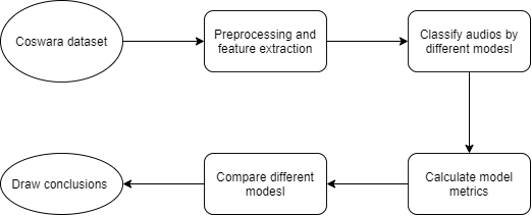
\includegraphics[width=.8\textwidth]{jiabao.png} % requires the graphicx package
    %\includegraphics[width=1\textwidth]{} % requires the graphicx package
    %\caption{\textbf{DNA甲基化和DNA羟甲基化谱的基因组规模分析方法}:目前研究使用的主要方法可分为基于限制酶的方法、基于重亚硫酸钠的方法和基于生物亲和力的方法}
    \label{fig_methyltech}
    %\vspace{0.8cm} % 用来调整和下方文字的间距
 \end{figure}


\subsection{Modeling work}
After the data preprocessinbg work, the classification models can be applied to the formatted
dataset to explore the potential subgroups of the COVID-19 cough audio. \\

\subsubsection{VAE}
For the variational autoencoders (VAE) model,
the encoder and the decoder are included in the model, which are popular model in the audio and
music areas\cite{girin2020dynamical}. The VAE model may also be able to classify our coswara dataset with multiple
clinical labels, and the VAE model will be implemented by packages such as pytorch and keras.

\subsubsection{GRU}
The GRU (Which stands for the gated recurrent unit) was proposed by the reference\cite{cho-etal-2014-properties}, it can make each recurrent
 unit adaptively capture dependencies of different time scales. The GRU has gating units which
 modulate the information flow inside the unit, however, it does not have any separate memory cells.
 Based on the experiment of \cite{Wang2nd}, the GRU mostly achieves comparable performance to the LSTM, sometimes
 even better performance on some datasets in terms of convergence in CPU time and parameter updates and
 generalization.

\subsubsection{RNN}
Compared to Convolutional Neural Networks (CNNs), Recurrent Neural Networks (RNNs) can better
model sequences of data since they are able to handle a variable-length sequence input.
In recent research work\cite{Yang1st,Yang2nd}, RNNs have already been adopted for COVID-19 cough classification.
A Gated Recurrent Unit (GRU) is a gating mechanism in RNNs\cite{Wang2nd}, which is similar to long
short-term memory (LSTM) but has fewer parameters. It has been shown that GRU can achieve better
performance on certain smaller and less frequent datasets\cite{Yang4th}. In this project, we will include
GRU model in the comparison to evaluate its performance on COVID-19 cough classification.
Similar to RNNs, transformer\cite{Yang5th} is designed to handle a variable-length sequential input data.
This machine learning model has been widely used in many fields, such as computer vision and
natural language processing. The key of its success is the adoption of the attention mechanism,
which differentially weighs the significance of each part of the input data and empower the model
to focus on important areas. Without using any RNN structure, transformer can achieve dominant
performance when handling the sequential data. We will also apply the transformer to COVID cough
classification to evaluate its performance.

\subsubsection{VGGish}
VGGish\cite{Chao1st} is an audio classification model that adopts the structure of VGG\cite{Chao2nd}, which is a
convolutional neural network originally used for image classification. VGG was the first runner-up of
ILSVR2014 in the ImageNet classification task. There are slight modifications to the architecture of
VGGish compared to that of VGG, including the input size being changed to better meet the needs of
log mel spectrogram inputs, dropping the last group of convolutional and maxpool layers, and using
a 128-fully connected layer instead of a 1000-fully connected layer. As VGGish was trained on a large
collection of audio data, AudioSet\cite{Chao3rd}, VGGish is commonly used as a feature extractor to convert
raw audio inputs to 128-D embeddings. The pre-trained weights are also publicly available. \\

\noindent
There has been previous work adopting VGGish extracted features, handcrafted features, and combined
 features to classify respiratory sounds\cite{Chao1st}. There has also been previous work on lung sound
 recognition using VGGish and bidirectional GRU\cite{Chao5th}. In this project, we aim to leverage VGGish to
 distinguish between covid cough sounds and non-covid cough sounds.

\subsubsection{Transformer-CP}
Transformer-CP is a model enabling contrastive pre-training. A contrastive learning method can
benefit from large batch size and can avoid overfitting problems in the downstream network. By
introducing a random masking mechanism, the feature encoder would be more robust. The masking
generator generates a masking matrix 𝑀 with a specific masking rate. Based on the masking matrix
and the masking rate, some of the inputs are randomly masked and removed from the attention calculation
in the Transformer. The loss function used in this phase for contrastive learning is a multi-class
cross-entropy function working together with the similarity metric.\\


\subsection{Model comparsion}
\noindent
In the end, we will compare different models (such as VAE, GRU, RNN, etc) by the same metrics to evaluate this classification
problem, such as the common metrics\cite{hossin2015review}. The preprocess methods, models and classification metrics will be
implemented by us and we will also compare the models by the metrics, which is a work contributed by us equally.
Eventually, by comparing the performance of the models which
 we have implemented, the potential suggestions on diagnosis methods or detection COVID-19 by audio
 information may also be given in the final part of our project.



\newpage
\bibliography{KDD}
\end{document}
